\documentclass[table]{article}

\usepackage[table]{xcolor}
\usepackage{multirow}
\usepackage{amsmath}
\usepackage{tabularx}
\usepackage{textcomp}
\usepackage{amssymb}
\usepackage{tikz}
\usepackage{bytefield}
\usetikzlibrary{calc,positioning,arrows,fit}
\usepackage[margin=2cm]{geometry}
\usepackage{graphicx}
\usepackage[utf8]{inputenc}
\usepackage{listings}
\usepackage{enumitem}
\usepackage{multicol}
\usepackage[colorlinks,urlcolor=blue,hypertexnames=true]{hyperref}
\usepackage{ifthen}
\usepackage{fancyhdr}
\usepackage{subcaption}
\usepackage{soul}
\usepackage{algpseudocode}
\usepackage{algorithm}
\usepackage{algorithmicx}
\usepackage{graphicx}

\usepackage{listings}
\usepackage{color}

\definecolor{dkgreen}{rgb}{0,0.6,0}
\definecolor{gray}{rgb}{0.5,0.5,0.5}
\definecolor{mauve}{rgb}{0.58,0,0.82}

\lstset{frame=tb,
  language=Java,
  aboveskip=10mm,
  belowskip=10mm,
  showstringspaces=false,
  columns=flexible,
  basicstyle={\small\ttfamily},
  numbers=none,
  numberstyle=\tiny\color{gray},
  keywordstyle=\color{blue},
  commentstyle=\color{dkgreen},
  stringstyle=\color{mauve},
  breaklines=true,
  breakatwhitespace=true,
  tabsize=8
}

\title{Theory of Computation - Assignment 6}
% \author{}

\pagestyle{fancy}
\fancyhf{}
\lhead{Theory of Computation - Assignment 6}
% \rhead{Ian Abuaf Pelo}
\rfoot{\thepage}

\begin{document}
\maketitle
\section{INTRODUCTION}

\leftskip=0.5in 
The clique problem is the computational problem of finding cliques in a graph. Given an undirected graph with N nodes and E edges and a value K, the task is to print all set of nodes which form a K size clique. 

\begin{center}
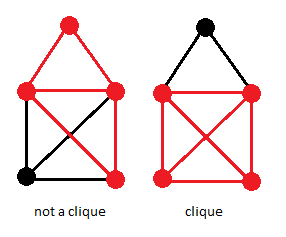
\includegraphics[scale=0.7]{MrlSG.png}
\end{center}

A clique C of a graph G is usually defined as a subset of the vertex set of G (V(G)) such that every pair of distinct vertices in C is adjacent in G (That is, two vertices u,v $\in$ C and u$\neq$v implies that u,v $\in$ E(G)). In other words, a subset of the vertex set of G is a clique if and only if its induced subgraph is a complete graph, that is if all distinct vertices are joined by and edge.\newline
 
The input of the k-clique problem is an undirected graph and a number k. 
An undirected graph is formed by a finite set of vertices and a set of unordered pairs of vertices, which are called edges. he output is a clique with k vertices, if one exists, or a special value indicating that there is no k-clique otherwise. \newline

\leftskip=0.0in 
\section{REDUCTION: 3-SAT TO K-CLIQUE}
\subsection{3-SAT}

\leftskip=0.5in 
3-SAT, or the Boolean satisfiability problem (sometimes called propositional satisfiability problem and abbreviated SATISFIABILITY, SAT or B-SAT), is the problem of determining if there exists an interpretation that satisfies a given formula in Boolean algebra (with unknown number of variables) whether it is satisfiable, that is, whether there is some combination of the (binary) values of the variables that will give 1.
In other words, it asks whether the variables of a given Boolean formula can be consistently replaced by the values TRUE or FALSE in such a way that the formula evaluates to TRUE. If this is the case, the formula is called satisfiable. On the other hand, if no such assignment exists, the function expressed by the formula is FALSE for all possible variable assignments and the formula is unsatisfiable.\newline

\leftskip=0.0in 
\section{K-CLIQUE TO SAT}

\leftskip=0.5in 
Given a graph G=(V,E) and a number k, we will have variables $x_{iv}$ for every 1$\leq$i$\leq$k and every v$\in$V. You should think of $x_{iv}$ as stating that v is the $ith$ vertex in the clique. We want to encode the following constraints:

\begin{enumerate}\leftskip=0.8in 
\item 	For each i, there is an $ith$ vertex in the clique: \[\forall i\in \{1,\dots,k\}, \; x_{i1} \lor x_{i2} \lor x_{i3} \lor \dots \lor x_{iv}\]
\item   For each i,j the $ith$ vertex is different from the $jth$ vertex: \[\forall v\in V, \forall(i,j)\in \{1,\dots,k\}, \; \neg x_{iv} \lor \neg x_{jv}\]
\item 	For each i,j, the $ith$ vertex is connected to the $jth$ vertex: \[\forall v\in V, \forall(i,j)\in \{1,\dots,k\}, \; \neg x_{iv} \lor x_{ju_1} \lor \dots \lor x_{ju_m}\], s.t. $u_{1,\dots,m}$ are the neighbours of $v$.
\end{enumerate}

\leftskip=0.5in
If we take all these clauses together, we get a CNF which states that "the $x_{iv}$ encode a k-clique in G". This CNF is satisfiable if and only if G contains a k-clique.
In order to get a 3CNF, we need to convert the constraints of the first kind into 3-clauses. If the vertices are $v_1$,...,$v_n$, we replace $V_{v \in V} x_{iv}$ with:

\begin{center}
$x_{iv_1} \lor x_{iv_2} \lor y_{iv_2} $ \newline
$\neg y_{iv_2} \lor x_{iv_3} \lor y_{iv_3} $ \newline
$\neg y_{iv_3} \lor x_{iv_4} \lor y_{iv_4} $ \newline
... \newline
$\neg y_{iv_{n-2}} \lor x_{iv_{n-1}} \lor x_{iv_n} $ \newline
\end{center}

\leftskip=0.5in 
Here the $y_{iv}$ are new variables. This set of clauses is equivalent to the original clause $x_{iv_1} \lor x_{iv_2} \lor ... \lor x_{iv_n} $.

\leftskip=0.0in  
\section{ALGORITHM}

\leftskip=0.5in  
We have found a solution, in which, for a complete graph with v vertices:
\begin{enumerate}\leftskip=0.8in 
\item We take all unconnected pair of vertices.
\item For each, at least one of them doesn't belong in a clique (If both did, it wouldn't be a clique since the two don't connect).
\item Then, check that at least k vertices are part of the clique.
\end{enumerate}

\leftskip=0.0in  
\section{CODE}

\leftskip=0.5in  
To solve the problem, we have created the following functions.
The \textit{solve()} function will create clauses for pairs of vertices that are not connected to each other. It will do this in the following way: \newline

\begin{itemize}\leftskip=0.8in
\item First we check that the size (which we have stored in the variable called "size") is equal to 0. If it is, we will return an error message since the network must contain at least one vertex (otherwise it is unsolvable and makes no sense).
\item If it is not, we continue.
\end{itemize}
 
\leftskip=0.5in
We will consider the vertices as a triangular matrix, in which in the first row will appear the connections that vertex 0 has, in the second row those of vertex 1, and so on until the last vertex (being 0 not connected with another vertex and 1 connected with another vertex).\newline

For example, if we have 5 vertices and vertex 0 is connected to vertices 1 and 3, the first column of the matrix will be the following: 0 1 0 1 0 0

Therefore, we will go through the matrix row by row and column by column, i.e. element by element. 

For each element of the matrix:

\begin{itemize}\leftskip=0.8in
\item If it is 1, i.e. the vertices are connected to each other, we continue.
\item If it is 0, i.e. the vertices are not connected, we create a clause, since that row and that column (i.e. that pair of vertices) cannot be in the clique.
\end{itemize}

\leftskip=0.5in
Then we call the function \textit{recursiveClaurses()}, this function computes the rest of the clauses to make sure that at least k variables are true.

Once we have this, we will join the clauses created for the unconnected vertices with the clauses for the connected vertices, which will form our solution.

We will pass these clauses created for a given size to the \textit{satSolve()} function. If it does not find a solution, no solution will be displayed, but if it does, it will be displayed. There may be more than one possible clique within a network for a given size k. This function will display one of the possible solutions at random.\newline

The code of the function is as follows:

\begin{lstlisting}
    Function solve() {
	let size = instanceVertexCount;
    	let clauses = []
        if (size == 0) throw("Graph must contain at least 1 vertex")
        for (row in instance) {
            for (col in instance[row]) {
                // For each possible combination of vertices
                if (!instance[row][col]) {
                    // If there is no edge create a clause
                    // "Either row or col are not in the clique"
                    clauses.push([-(parseInt(row)+1), -(parseInt(col)+1)])
                }
            }
        }
        let others = recursiveClauses(size - k + 1)
        clauses = clauses.concat(others)
        let solution = satSolve(size, clauses)
        if (!solution) return solution 
        return solution.filter(i => i>0).map(i => i-1)
    }

\end{lstlisting}

As we have already said, the function \textit{recursiveClaurses()} computes the rest of the clauses to make sure that at least k variables are true. 
We will call this function recursively, creating a vector for each iteration in which we will add clauses for each vertex, until we reach the last vertex where we will stop the recursion.

The code of the function is as follows:

\begin{lstlisting}
    function recursiveClauses(stop, v = [], j = 0) {
    let out = []
        if (v.length == stop) return [v]
        for (let i = j; i < instanceVertexCount; i++) {
            next = [...v]
            next.push(i+1)
            out = out.concat(recursiveClauses(stop, next, i+1))
        }
        return out
    }

\end{lstlisting}


\section{TEST CASES}

\end{document}
